\subsection{Ca sử dụng thêm vị trí cho ảnh}

\vspace{0.5cm}

\noindent 
\begin{tabularx}{\linewidth}{| l | X |} 
\hline 
\textbf{Mô tả} & Người dùng thêm vị trí cho ảnh. \\
\hline 
\textbf{Luồng cơ bản} & 1. Người dùng chọn nút thêm vị trí cho ảnh ở thanh công cụ dưới màn hình. \newline
                       2. Hệ thống điều hướng đến trang thêm vị trí cho ảnh. \newline
                       3. Hệ thống hiển thị hộp thoại cấp quyền thông tin vị trí hiện tại. \newline
                       4. Người dùng cấp quyền truy cập vị trí hiện tại. \newline
                       5. Hệ thống lấy thông tin vị trí hiện tại của người dùng và hiển thị trên bản đồ. \newline
                       6. Người dùng chọn vị trí trên bản đồ. \newline
                       7. Người dùng bấm nút xác nhận để thêm vị trí cho ảnh. \newline
                       8. Hệ thống lưu vị trí cho ảnh và hiển thị thông báo thành công. \\
\hline
\textbf{Luồng thay thế} & - Người dùng tìm kiếm địa điểm thay vì tự chọn vị trí thủ công trên bản đồ. \newline
                          - Hệ thống không lấy được dữ liệu địa điểm từ vị trí người dùng chọn trên bản đồ. \\
\hline
\textbf{Tiền điều kiện} & - Người dùng đã đăng nhập vào hệ thống. \newline
                          - Có ít nhất 1 bức ảnh đã tải lên trong thư viện. \\
\hline
\textbf{Hậu điều kiện} & - Người dùng có thể xem vị trí hiện tại của bản thân. \newline
                          - Người dùng có thể xem thông tin chi tiết của vị trí vừa chọn. \\
\hline 
\textbf{Yêu cầu phi chức năng} & - Hệ thống lấy dữ liệu của địa điểm không quá 2s. \newline
                           - Hệ thống lấy được dữ liệu hiện tại vị trí người dùng (nếu được cấp quyền). \\
\hline 
\end{tabularx}

\vspace{0.8cm}

\noindent 
\begin{tabular}{| c | c |}
    \hline
    \textbf{Biểu đồ hoạt động} & \textbf{Quan hệ} \\ 
    \hline
    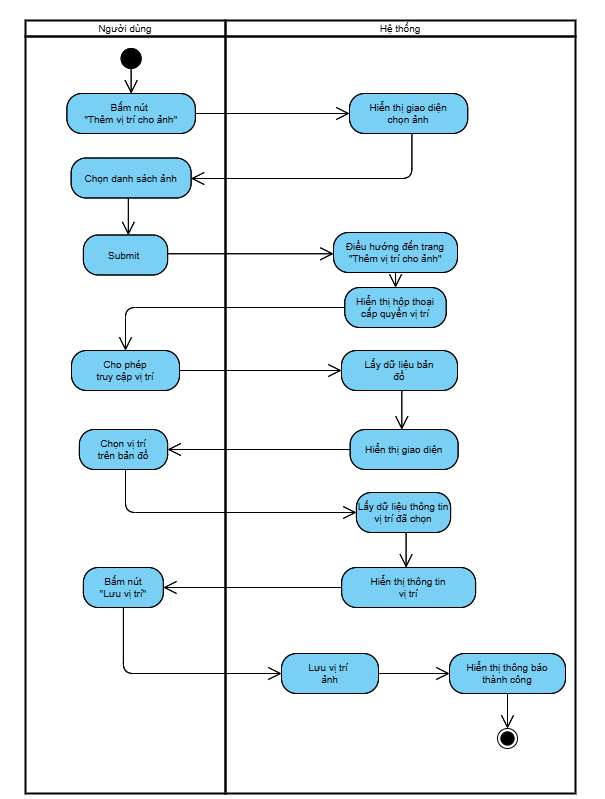
\includegraphics[width=0.6\linewidth]{figures/c3/3-3-15-activity-diagram.png} 
    &  
    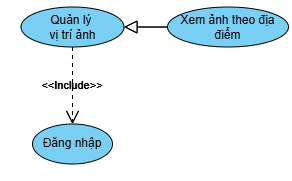
\includegraphics[width=0.35\linewidth]{figures/c3/3-3-15-relationship.png} \\ 
    \hline
\end{tabular}

\begin{figure}[H]
    \centering  
    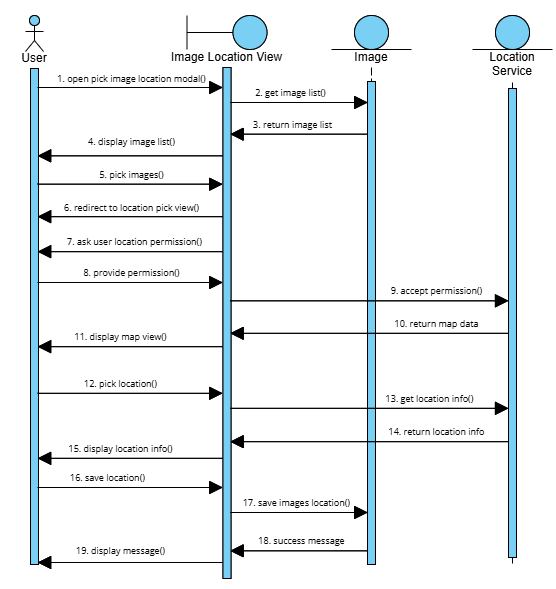
\includegraphics[width=1\textwidth]{figures/c3/3-3-15-sequence-diagram.png}
    \caption{Biểu đồ tuần tự ca sử dụng thêm vị trí cho ảnh.}
    \label{fig:3-3-15-sequence-diagram}
\end{figure}